\subsection{What is Artificial Intelligence?}
Artificial Intelligence (AI) refers to the simulation of human intelligence in machines that are programmed to perform tasks that normally require human intelligence such as learning, problem-solving, decision-making, perception, language understanding, and more\cite{ISSN-2456-2165}. AI systems use algorithms and statistical models to analyze data, recognize patterns, and make predictions, without explicit instructions from human operators.

\subsection{Limitations of Artificial Intelligence}
Although artificial intelligence (AI) has made significant advancements in recent years, there are still some limitations to the technology. Some of the limitations are:
\begin{itemize}
	\item \textbf{Lack of Common Sense:} AI systems lack the common sense that humans have, which can make it difficult for them to understand complex situations and make appropriate decisions.
	\item \textbf{Limited Creativity:} AI systems are designed to operate within the parameters set by their algorithms and data, which limits their ability to generate truly creative solutions or ideas.
	\item \textbf{Lack of Emotional Intelligence:} AI systems are not capable of experiencing emotions, which limits their ability to understand and respond to emotional cues in human interactions.
\end{itemize}
Limitations of AI highlight the need for continued research and development to address these issues and improve the capabilities of these systems.

\subsection{What is Emotional Intelligence?}
Emotional Intelligence (EI) refers to the ability to recognize, understand and manage one's own emotions as well as the emotions of others. It involves being able to use emotional information to guide thinking and behavior, and to navigate social situations effectively\cite{ISSN-2456-2165}.

EI is often described as having four components: self-awareness, self-management, social awareness, and relationship management. Self-awareness involves recognizing and understanding one's own emotions, strengths, and weaknesses. Self-management involves being able to regulate one's own emotions and behaviors in response to different situations. Social awareness involves recognizing and understanding the emotions of others, as well as the social norms and expectations of different situations. Relationship management involves using emotional information to communicate effectively, build and maintain relationships, and resolve conflicts.

EI is considered an important factor in personal and professional success, as it can help individuals navigate social interactions, build strong relationships, and manage stress and challenges effectively.

\subsection{Emotional Artificial Intelligence}
Emotional Artificial Intelligence (EAI) is the ability of AI systems to recognize, understand, and respond appropriately to human emotions. It is an emerging field of AI that focuses on building machines that can perceive, interpret, and express emotions similar to human beings. 

Emotional AI uses various techniques such as natural language processing, sentiment analysis, and facial recognition to detect emotions in human interactions. These techniques are then used to train algorithms and models that can predict and respond to human emotions in real-time.

Emotional AI has numerous potential applications, such as improving customer service, enhancing human-robot interactions, and providing mental health support.

\subsection{Why Truly Intelligent Machines Need Emotions?}
Many machines are in our household items such as kitchen, bedroom, which are artificially intelligent to help us with our daily tasks, however, they are emotionally unintelligent to adapt to our fulfillment. If one desires an Artificial Intelligence, the Artificial Intelligence should be able to adapt to the individual's state of mind. At the present time, many leading companies have expanded the idea of Emotional Artificial Intelligence into their AI systems.\cite{ISSN-2456-2165}.

The need of EIM's are can be seen due to their numerous applications which are expanding rapidly.
Some of the common applications of EIM's include:
\begin{itemize}
	\item \textbf{Social Media:} They can be used in social media to analyse user's emotions and provide more personalized content.
	\item \textbf{Business Intelligence(BI) \& Operational Research(OR):} EIM's are more intelligent than the traditional machines as a result they can help in Decision Making which is involved in Business Intelligence \& Operational Research.
	\item \textbf{Human Resources:} In human resources to analyse employee's emotions and improve the work environment and productivity.
	\item \textbf{Development of Machine Ethics \& Computational Morality:} Emotional AI can play a vital role in the development of machine ethics and morality. It will allow machines to understand and respond to human emotions, which is an important component of ethical and moral decision-making.
	\item \textbf{Human-Computer Interaction(HCI):} Emotional AI is extremely helpful in HCI, as it enables computers to understand and respond to human emotions, making the interaction more natural, intuitive, and empathetic. Here are some ways in which Emotional AI can be useful in developing machine ethics and morality:
	\begin{itemize}
		\item \textbf{Understanding Human Emotions:} EAI can help machines to understand human emotions, which is an important component of ethical decision-making. For example, a machine that can detect when a human is experiencing fear or pain could adjust its behavior accordingly to avoid causing harm.
		\item \textbf{Ethical Decision-Making:} EAI can help machines to make more ethical decisions by taking into account human emotions and responses. For example, a self-driving car that can detect when a passenger is feeling anxious or stressed could adjust its driving style to provide a safer and more comfortable ride.
		\item \textbf{Morality and Empathy:} Emotional AI can help machines to exhibit more empathy towards humans, which is an important component of moral decision-making. For example, a robot that can detect when a human is feeling sad or lonely could provide comfort or companionship.
		\item \textbf{Human-Machine Collaboration:} Emotional AI can help facilitate collaboration between humans and machines by allowing machines to understand and respond to human emotions. This could lead to more effective and productive collaborations, as well as greater trust between humans and machines.
	\end{itemize}
	\item \textbf{Customer Service:} EAI can be used in customer service to understand customer's emotions and respond accordingly, improving customer satisfaction. It can also be used in getting customer reviews, feedbacks \& and conducting surveys.
	\item \textbf{Healthcare:} EAI could be very useful in healthcare sector to detect patient's emotions and provide appropriate treatment and care. They could be a great blessing for the treatment of psychic patients and for counselling of persons suffering form depression \& anxiety or even having suicidal tendency.
	\item \textbf{Education:} EAI can be used in education sector to improve the effectiveness of teaching by understanding the emotional state of the students and adapting the teaching method accordingly.
	\item \textbf{Marketing, Sales \& Advertisement:} EAI can be used in marketing to analyze customer's emotions and tailor marketing messages to maximize their impact which leads in increment of sales conversion rate.
	\item \textbf{Art \& Culture:} AI which can generate creative artistic content like Melodies \& Progressions in Music, Paintings \& Poetry is currently based on logical reasoning. By the development of Emotional AI, generation of this type of content can reach the next level of the arts which can also be used by the artists as a reference for their work.
	\item \textbf{Media \& Communication:} EAI has a huge potential to do great in the field of media as it can be used as a NEWS anchor or an interactive agent which can communicate with their listeners emoitionally.
	\item \textbf{Entertainment:} Emotionally Intelligent Machines can be used in the entertainment industry to create more immersive experiences for users by understanding their emotional responses, in gaming industry to create more engaging games that respond to the player's emotions also create the dynamic gaming environment accordingly, in movies industry to create ambience, environments and also in writing scripts.
\end{itemize}
\subsection{Convergence, Divergence and Belief Systems of AI}
\subsubsection{Stability and Unstability}
\subsection{Conscious, Subconscious \& Unconscious of Aritificial Intelligence}
\subsubsection{Recurrent Neural Networks as Consciousness of AI}
\subsubsection{Feed Forward Networks as Subconscious of AI}
\subsubsection{How to design the Unconscious of AI?}
\subsection{Emotion Dynamics}
\subsection{The Butterfly Effect \& Chaos Theory}
Richard A. Anthes in 2022 by his paper "Predictability \& Predictions" showed his experiences with predictability theory and weather predictions began as an undergraduate student at the University of Wisconsin in Madison in the early 1960s. His interest in numerical simulations led to the development of a simple nonlinear one-dimensional gravity wave model and later a nonlinear, baroclinic, three-dimensional model of the tropical cyclone. His experiences highlighted the challenges of numerical and physical instabilities in weather prediction models \cite{atmos13081292}. \cite{encyclopedia2030084}
\subsection{Quantum Level V/S Cosmic Level}
\subsubsection{Microscopic V/S Macroscopic}
\subsection{Plutchik's Wheel of Emotions}
\begin{figure}[H]
	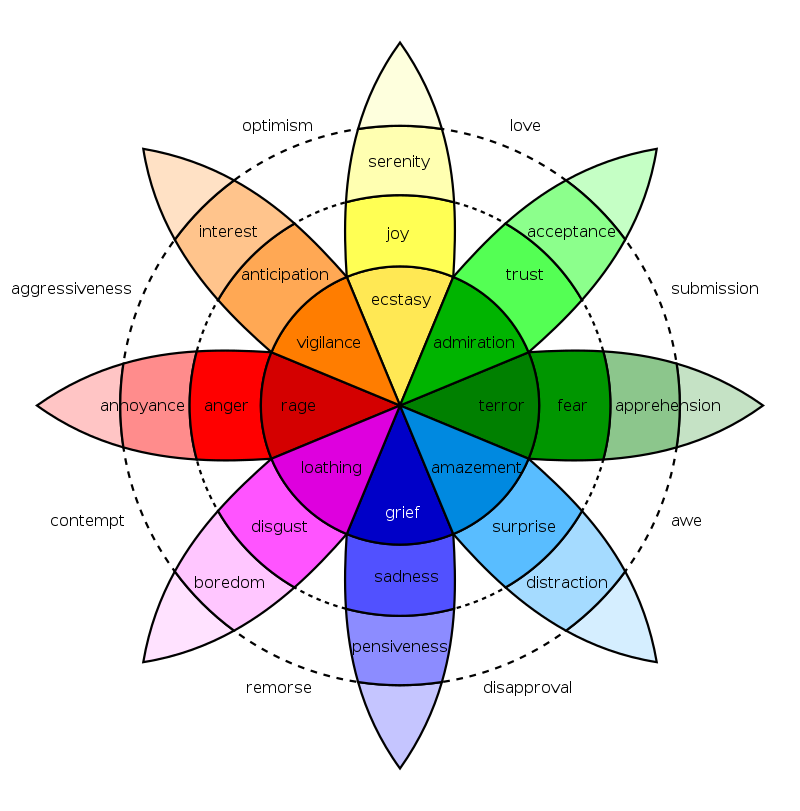
\includegraphics[width=\columnwidth, keepaspectratio]{Plutchik'sWheelofEmotions.png}
	\caption{Plutchik's Wheel of Emotions}
	\label{Fig:fig1}
\end{figure}
Figure \ref{Fig:fig1} shows PWOE.
\subsection{Ancient Vedic Astrology}
A Brief History of Ancient Vedic Astrology
\subsubsection{Classification of Vedic Astrology}
\subsubsection{Surya Siddhanta}
\subsubsection{Vrihat Samhita}
\subsubsection{Brihat Parashar Hora Shastra}
101 Chapters
4500 Verses
\subsubsection{Significance of Planets}
\begin{sanskrit}
	\begin{center}
		देवेज्यो ज्ञानसुखदो भृगुर्वीर्यप्रदयकः।\\ऋषिभिः प्राक्‌तनैः प्रोक्तश्छायासूनुश्च दुःखदः॥३:१४॥\cite{BrihatParasharHoraShastraVol1}
	\end{center}
\end{sanskrit}